\section{System-Level Framework}
\label{sec:exec_time_prediction.system}

This section describes the overall framework and operation of our
prediction-based controller.

\subsection{Programmer Annotation}

% Programmer annotation
\begin{figure}
  \begin{center}
    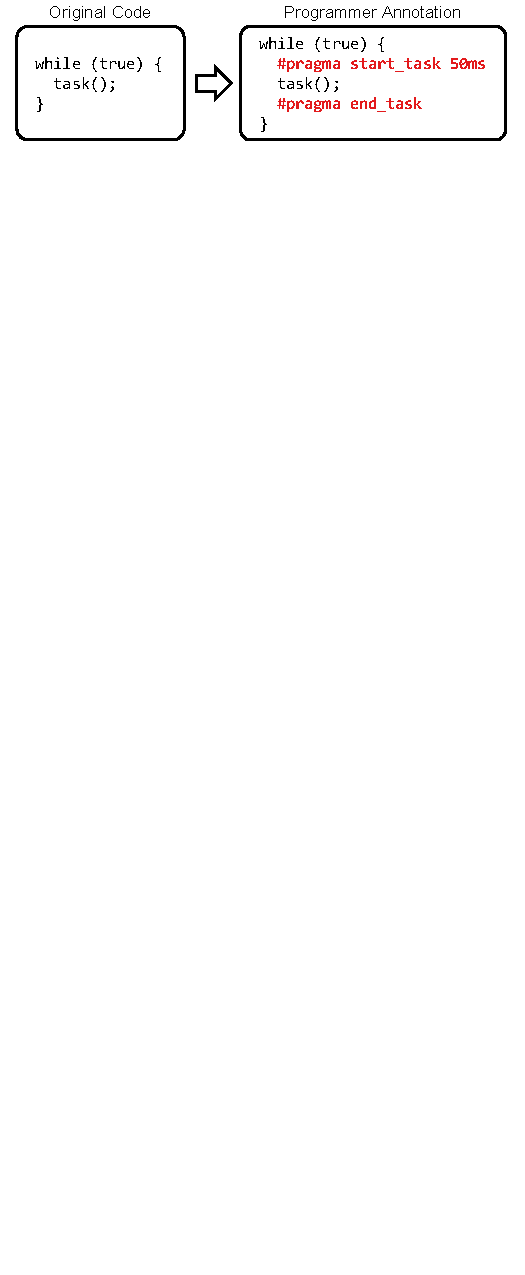
\includegraphics{exec_time_prediction/figs/programmer_annotation.pdf}
    \caption{Example of programmer annotation to mark task boundaries and time
    budgets.}
    \label{fig:exec_time_prediction.system.programmer_annotation}
  \end{center}
\end{figure}

In order to identify tasks and their time budgets, programmer annotation is
required. The programmer must annotate the start and the end of a task and the
desired response-time requirement.
Figure~\ref{fig:exec_time_prediction.system.programmer_annotation} shows an
example of this annotation.  For ease of analysis and to ensure that tasks that
start always end, we require the start and end of a task to be within one
function.  Arbitrary code paths can be modified to fit this model by using a
wrapper function or re-writing the code. Multiple non-overlapping tasks can be
supported, though we only considered one task in the applications we tested.

\subsection{Off-line Analysis}

% High-level flow of framework
\begin{figure*}
  \begin{center}
    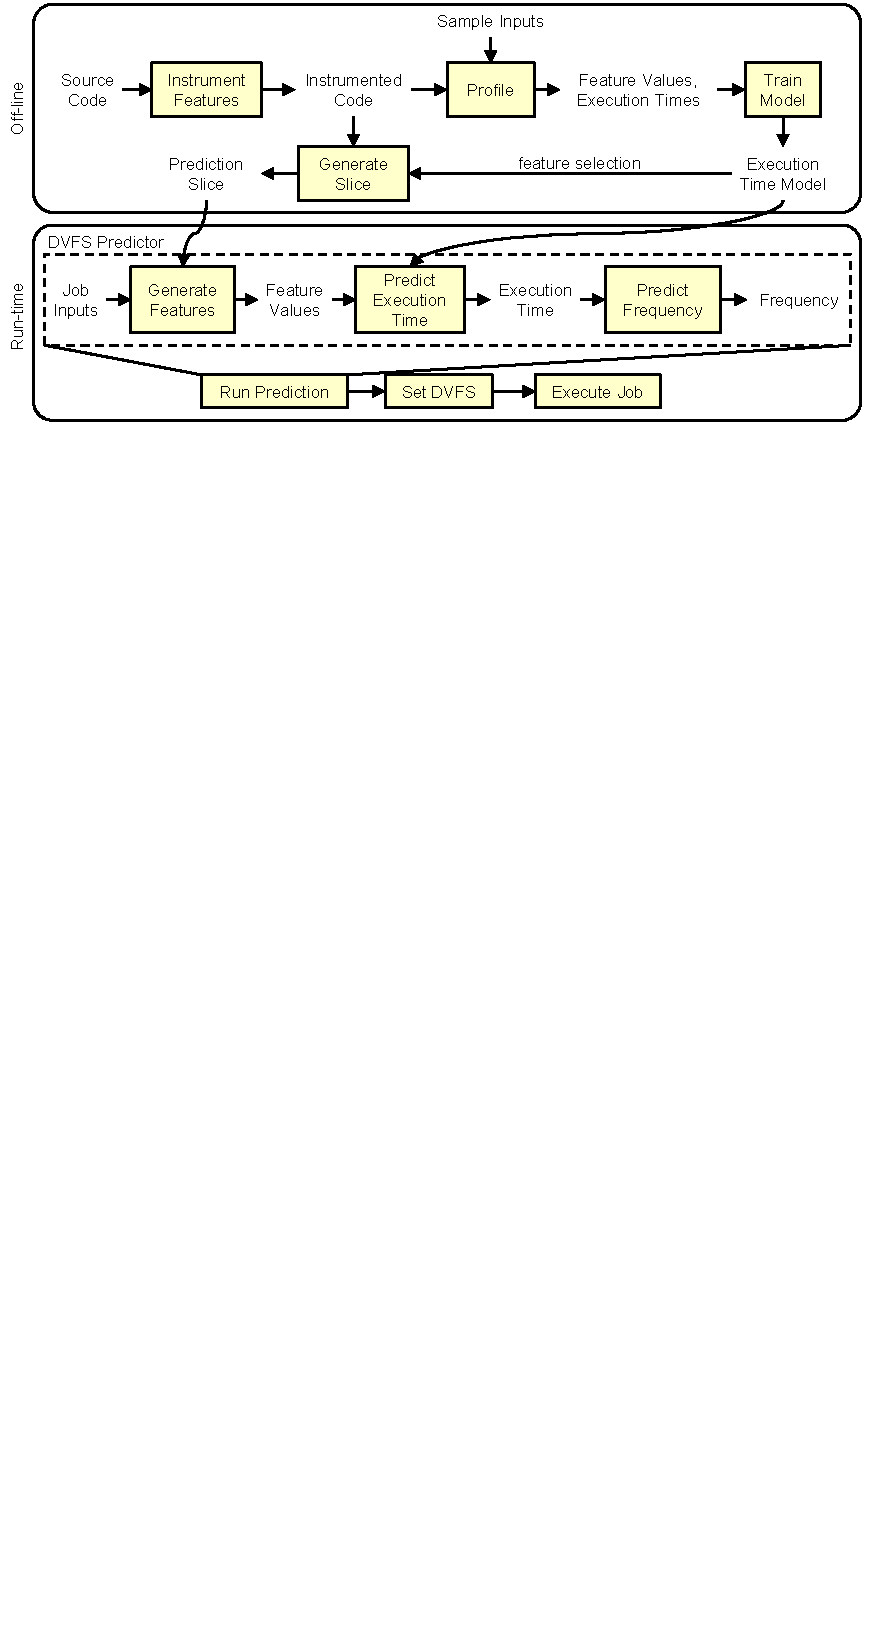
\includegraphics{exec_time_prediction/figs/high_level_flow.pdf}
    \caption{Overall flow for prediction-based DVFS control.}
    \label{fig:exec_time_prediction.system.high_level_flow}
  \end{center}
\end{figure*}

Figure~\ref{fig:exec_time_prediction.system.high_level_flow} shows the overall
flow of our framework for creating prediction-based DVFS controllers. Given
programmer annotation to identify tasks, we can automatically instrument these
tasks to record control flow features. Off-line, we profile these tasks in
order to collect traces of feature values and job execution times.  This is
used to train our execution time prediction model, as described in
Section~\ref{sec:exec_time_prediction.prediction.model}. Since execution time
depends on the specific hardware and platform that an application is run on,
profiling and model training needs to be done for the platform that the
application will be run on. For common platforms, the program developer can
perform this profiling and distribute the trained model coefficients with the
program. Alternatively, profiling can be done by the user during the
application's installation.

% Differences in slice features
\begin{table*}
  \begin{center}
    \begin{footnotesize}
    \begin{tabular}{|l|l|r|r|r|}

\hline
\multirow{2}{*}{\bf Platform} & \multirow{2}{*}{\bf Benchmark} & \multirow{2}{*}{\bf Feature Diff} & \multicolumn{2}{r|}{\bf Prediction Diff} \\ \cline{4-5}
& & & {\bf Average} & {\bf Max} \\ \hline\hline

\multirow{8}{*}{ARM-big}
& 2048         & --     & 0\%   & 0\%   \\ \cline{2-5}
& curseofwar   & --     & 0\%   & 0\%   \\ \cline{2-5}
& ldecode      & --     & 0\%   & 0\%   \\ \cline{2-5}
& pocketsphinx & --     & 0\%   & 0\%   \\ \cline{2-5}
& rijndael     & --     & 0\%   & 0\%   \\ \cline{2-5}
& sha          & --     & 0\%   & 0\%   \\ \cline{2-5}
& uzbl         & --     & 0\%   & 0\%   \\ \cline{2-5}
& xpilot       & -2, +1 & 0.1\% & 8.7\% \\ \hline\hline

\multirow{8}{*}{x86}
& 2048         & +67    & 0.4\% & 2.9\% \\ \cline{2-5}
& curseofwar   & --     & 0\%   & 0\%   \\ \cline{2-5}
& ldecode      & --     & 0\%   & 0\%   \\ \cline{2-5}
& pocketsphinx & +2     & 0\%   & 0\%   \\ \cline{2-5}
& rijndael     & --     & 0\%   & 0\%   \\ \cline{2-5}
& sha          & --     & 0\%   & 0\%   \\ \cline{2-5}
& uzbl         & -1     & 0\%   & 0\%   \\ \cline{2-5}
& xpilot       & +6, -8 & 0.7\% & 2.9\% \\ \hline 

\end{tabular}

    \end{footnotesize}
    \caption{Differences in features selected and predicted execution times for
    different platforms compared to an ARM-LITTLE platform.}
    \label{tab:exec_time_prediction.system.slice_differences}
  \end{center}
\end{table*}

The trained execution time model only requires a subset of all the features to
perform prediction. Thus, this information is used to eliminate code for
calculating unneeded features.  Program slicing is then used to create a
minimal code fragment to calculate the needed control flow features.  Note that
since the features needed depends on the training of the execution time
prediction model, which is platform-dependent, the features needed could vary
across platforms. However, we expect the features that are needed are
primarily a function of the task semantics (i.e., execution time variations
across control paths) rather than the platform it is run on. In fact, we
compared the predictions made for an x86-based (Intel Core i7) platform when
using the features selected for an ARM LITTLE-based ODROID-XU3 platform and for the
features selected for the x86 platform itself. We also compared using the ARM
big core compared to the LITTLE core on the ODROID-XU3 platform. 
Table~\ref{tab:exec_time_prediction.system.slice_differences} shows the
features that are added or removed in the prediction slices for these platforms
compared to the prediction slice generated for the ARM LITTLE core. In
addition, the differences in predicted execution times using the prediction
slice generated for the platform and using the prediction slice from the ARM
LITTLE core are shown. 
For the ARM big core, only one benchmark shows differences in features selected
with the resulting difference in prediction times being only 0.1\% on average.
For the x86-based platform, four benchmarks show differences in features
selected. In two of these cases, the predicted execution times are not
affected. In the remaining two cases, average differences in predicted
execution times are less than 1\%.
%For all but three of the
%benchmarks we tested, the features selected were exactly the same.  For one of
%these, the features selected by the x86 platform were a subset of those
%selected by the ARM platform and so the predicted times were exactly the same.
%For the remaining two benchmarks, the predicted times differed by less than
%3\%. 
Although we had to re-train the execution time model coefficients for these new
platforms, the same prediction slice was applicable across both platforms.

\subsection{Run-time Prediction}

% Slice operation choices
\begin{figure}
  \begin{center}
    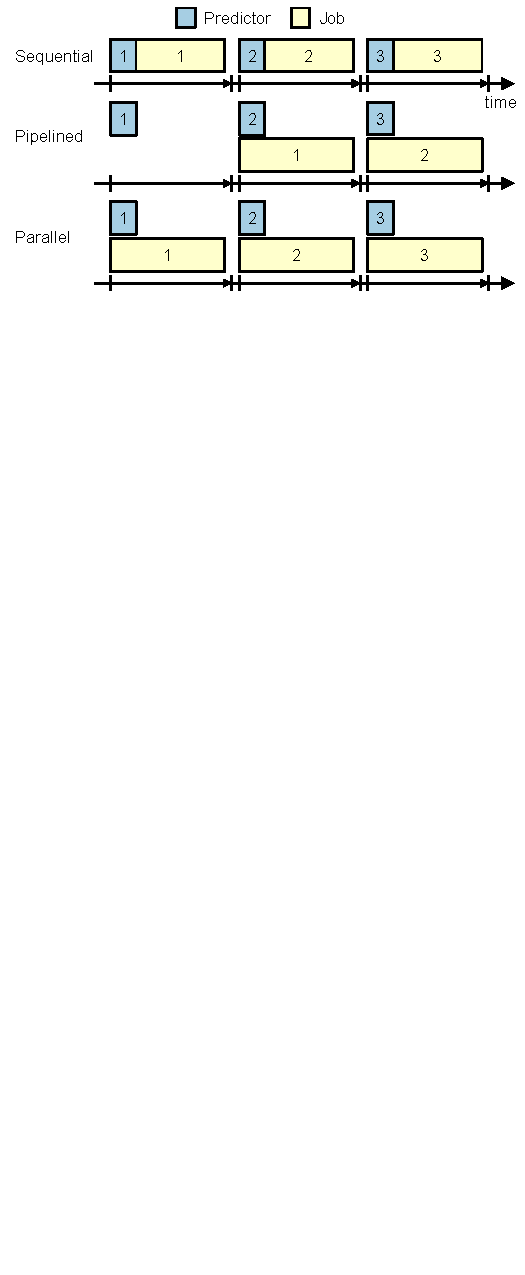
\includegraphics{exec_time_prediction/figs/predictor_operation.pdf}
    \caption{Options for how to run predictor.}
    \label{fig:exec_time_prediction.system.predictor_operation}
  \end{center}
\end{figure}

The prediction slice, execution time predictor, and frequency predictor are
combined to form the \emph{DVFS predictor} or simply \emph{predictor} There are
several options for how to run the predictor in relation to jobs.
Figure~\ref{fig:exec_time_prediction.system.predictor_operation} shows some of
these options.  The simplest approach is to run the slice just before the
execution of a job. This uses up part of the time budget to execute the predictor, as
mentioned in Section~\ref{sec:exec_time_prediction.prediction.dvfs}. However,
if this time is low, then the impact is minimal.

An alternative option would be to run the predictors and jobs in a parallel,
pipelined manner such that during job $i$, the predictor for job $i+1$ is run.
This ensures that the DVFS decision is ready at the start of a job with no
impact on time budget from the predictor. Due to the longer time budget,
running in a pipelined manner can save more energy than running in a sequential
manner. However, this assumes that
information needed by the prediction slice, specifically the job inputs and
program state, is ready one job in advance. This is not possible for
interactive tasks which depend on real-time user inputs or tasks which are not
periodic.

The predictor could also be run in parallel with the task. This avoids the
issue of needing input values early. In terms of time budget, this mode of
operation still reduces the effective budget by the predictor execution time.
However, part of the task also executes during the prediction time, so the
remaining work to be done is also reduced. Thus, this could still lead to
higher energy savings than running in a sequential manner.
Running in parallel also avoids the issue of side-effects
caused by the prediction slice that was discussed in
Section~\ref{sec:exec_time_prediction.prediction.features}. However, running in
parallel either requires forking off the predictor for each job or sharing data
with a dedicated predictor thread, both of which can introduce overhead.

For our target applications, we found that the execution time of the predictor
was low. Thus, we decided to run the predictor and task in a sequential manner
(i.e., ``Sequential'' in
Figure~\ref{fig:exec_time_prediction.system.predictor_operation})
For applications which require more complicated predictors, these alternative
operation modes may be beneficial.
